\chapter{The \texttt{VESUVIUS} Machine}
\label{chap:machine}

\section{Annealing Schedule}
The \texttt{VESUVIUS} machine on which our experiments were conducted is composed of 512 rf-SQUID superconducting qubits of the type described in \cite{qubit} \cite{dwave_nature}. It is the same phsyical machine as the larger of the two machines described in \cite{pudenz}.
As mentioned in Chapter \ref{chap:aqc} the form of the Hamiltonian we use for AQC is

\begin{displaymath}
	H_{tot} = f(t)H_i + g(t)H_f
\end{displaymath}

and the experiments were carried out with a transverse field of $f(0) \approx 33.8 $ GHz and a maximum normalized coupling value of $g(T) \approx 20.5$ GHz, and an annealing temperature of 17 mK.  These correspond to energies of $140 \mu$ eV and $85 \mu$ eV for the Hamiltonian components respectively and a thermal energy of $1.5 \mu$ eV.

\section{Resolution}
In addition to the graph-shape restrictions, the \texttt{VESUVIUS} machine cannot implement arbitrary physical Hamiltonians.  The machine can only implement fields and couplings as one of 15 distinct values: $-7/7, -6/7 \dots 5/7,6/7, 7/7$.  Call the largest coupling present in the problem Hamiltonian $C_{max}$, and the smallest \emph{magnitude} coupling $C_{min}$.  As our embedded Hamiltonians don't generally have a $C_{max}$ to $C_{min}$ distance of exactly 7, they must be manipulated to fit in this range.
First  all the field and coupling values are normalized into the range $[-1..1]$, and then each coupling is coerced to the nearest machine implemented value.
Unfortunately we don't know exactly how the coercion is done; it seems reasonable that each normalized coupling would be rounded to the nearest machine implemented coupling, but other schemes such as rounding toward or away from zero are possible.
The linear spacing of the machine implemented couplings implies that Hamiltonians with couplings that linearly fill the range from $-C_{max}$ to $C_{max}$ will be least affected by the coercing issue, while those Hamiltonians which have gaps between coupling values or other spacings will be most impacted by the effects of finite machine resolution.

\begin{figure}
	%\includegraphics
	\caption[Ideal vs. Physical Couplings]{This figure illustrates the difference between ideal and physically implemented couplings; the $\delta$-function like peaks are what ideal couplings would behave as, and the Gaussians what a real machine must implement.  The amount of overlap between the tails of the real couplings is dependent on the magnitude of the programming noise in the machine; the actual amount of overlap present in the \texttt{VESUVIUS} machine is unknown.}
	\label{fig:coupling_spread}
\end{figure}

\section{Programming Noise}
\label{sec:noise}
The resolution issue is exacerbated by the fact that there is some error in the programming of each coupling (or field).  Ideally one could imagine the physical coupling values implemented by the machine as a series of $\delta$-functions from $-C_{max}$ to $C_{max}$; however, because the couplings are non-ideal, the actual structure of the couplings looks more like Figure \ref{fig:coupling_spread}.  The magnitude of this error is uncertain; efforts are underway to quantify how much error is consistent with results from the machine \cite{aaron}.  If the overlap between adjacent programmable coupling values is large enough, then the Hamiltonian which is actually implemented during a particular run may have a different ground state then what we wished to program in; the larger the overlap, the more likely to get incorrect ground states.  The preliminary results in Chapter \ref{chap:prelim} suggest that the programming noise is in the neighbourhood of the machine coupling spacing, or large enough that it is possible for the programming noise to cause incorrect ground states.

\section{Inoperable Qubits}
Not every qubit on the \texttt{VESUVIUS} machine is functional all of the time.  As the machine is cooled to super-conducting temperatures, lines of magnetic flux can become trapped inside.  As some parts cool past the critical temperature before others, the Meissner effect forces magnetic flux out of the super-conducting regions into the regions which are still above the critical temperature.  If the regions of trapped flux are surrounded by super-conducting regions, there is no way for the trapped flux to escape and so it remains inside the machine, hindering the operation of whichever qubits it intersects.  As in the normal course of operation the machine is brought above super-conducting temperatures only for maintenance, the pattern of broken qubits can remain stable for long periods of time.  Figure \ref{fig:broken_qubits} shows the layout of the \texttt{VESUVIUS} machine, with the qubits that were inoperable for the duration of this study marked in red.

\begin{figure}
	\scalebox{0.80}{
		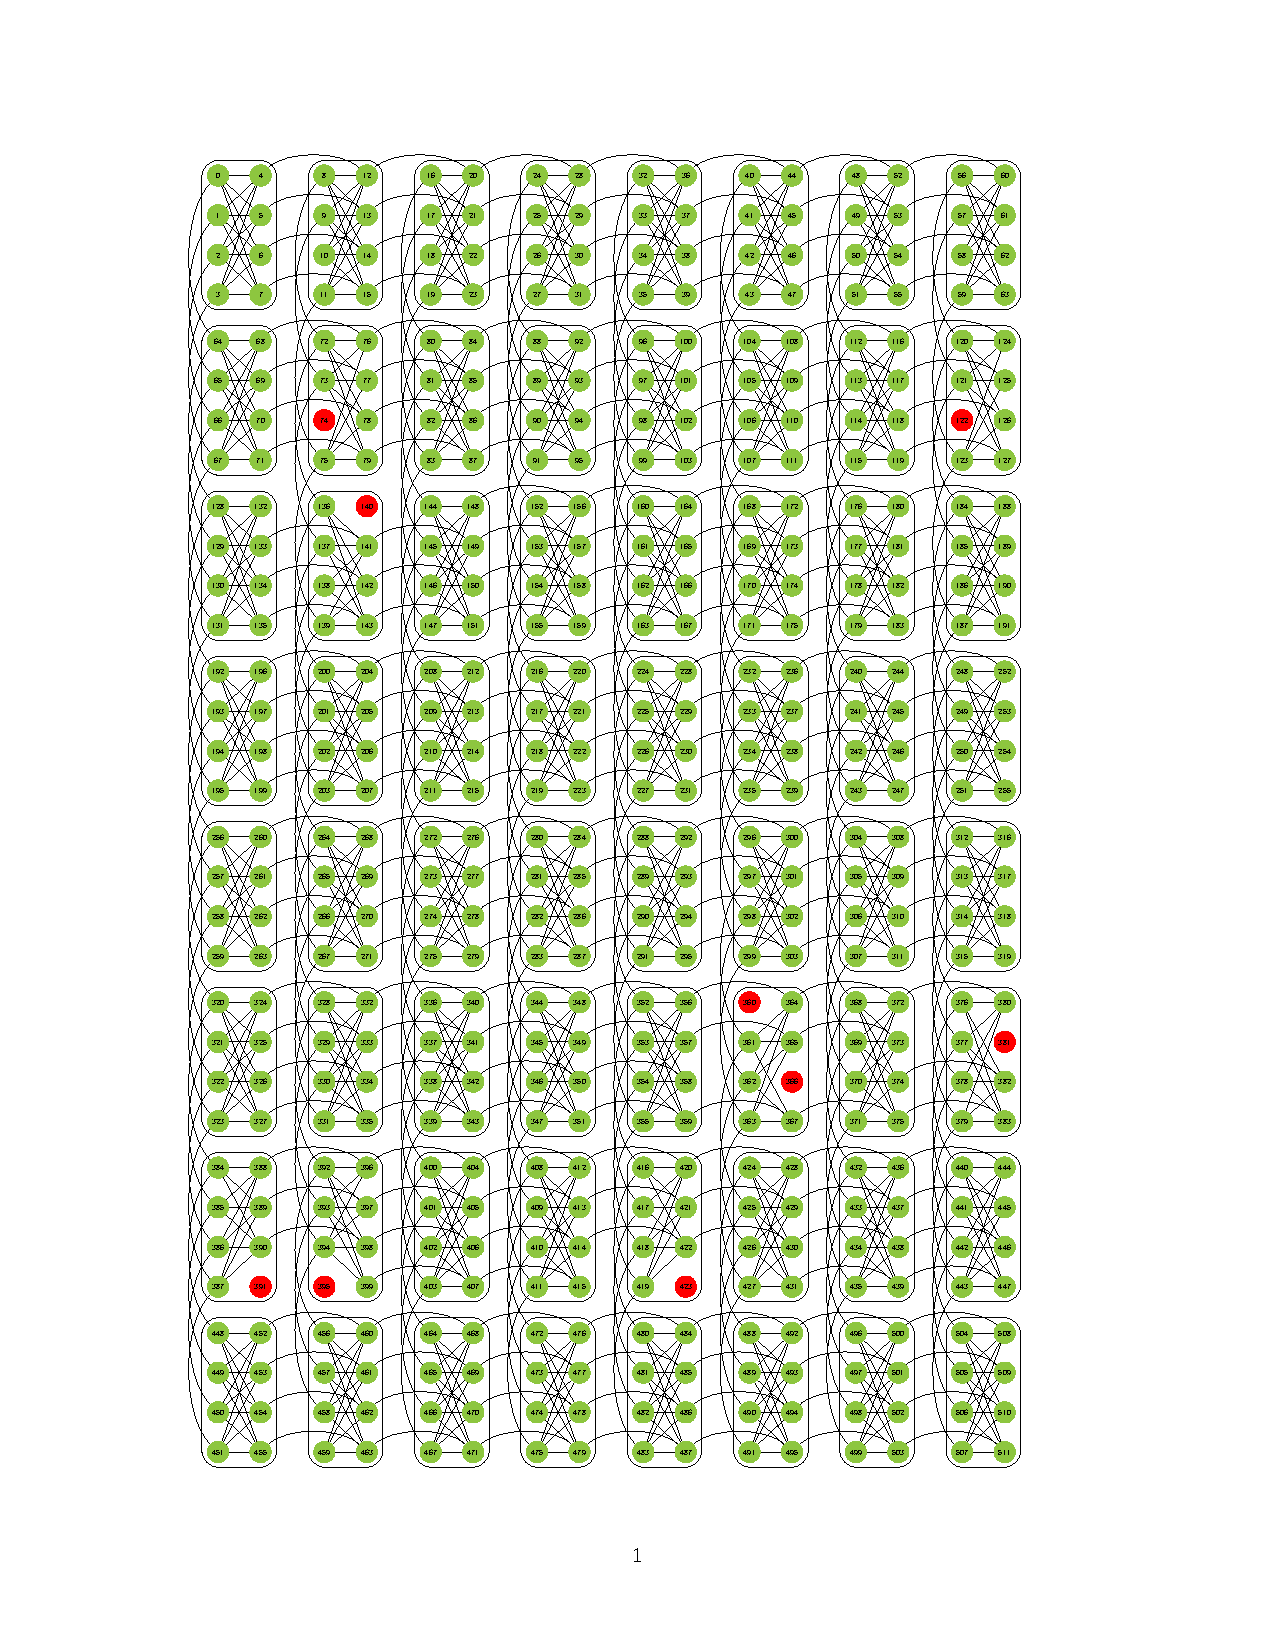
\includegraphics[bb= 0 0 8.5in 11in]{img/chimeraFig.pdf}
	}
	\caption[\texttt{VESUVIUS} Layout]{Diagram of the connectivity of the \texttt{VESUVIUS} machine showing the Chimera graph structure, with the qubits which were inoperable during the duration of this study marked in red.}
	\label{fig:broken_qubits}
\end{figure}
